\subsubsection{Formiranje evidencije o polaganju ispita}
\label{subsubsec:vozni park}
\begin{itemize}
  \item \textbf{Kratak opis}: Nadležni za zaposlene ima mogućnost da vodi evidenciju o polaganju praktičnog ispita. 
  Vodi računa o vremenu kad se održava ispit, instrukoru koji je zadužen za polaganje, kandidatu koji polaže ispit i o anketi koju kandidat popunjava na kraju ispita.

  \item \textbf{Učesnici}:
    \begin{itemize}
    \item Nadležni za zaposlene - korisnik sistema koji formira zapisnik o polaganju praktičnog ispita.
    \end{itemize}
  \item \textbf{Preduslovi}:
    \begin{itemize}
    \item  Nadležni za zaposlene je uspešno ulogovan na sistem auto škole.
    \item  Sistem je u funkciji.
    \item  Nadležni za zaposlene ima pristup internetu.
    \end{itemize}
  \item \textbf{Postuslovi}:
      \begin{itemize}
      \item  Nadležni za zaposlene je ažurirao evidenciju o ispitu.
      \item  Nadležni za zaposlene je ažurirao evidenciju o instruktorima, na osnovu anketa.
      \end{itemize}
  \item \textbf{Osnovni tok}:
      \begin{enumerate}
        \item Nadležni za zaposlene otvara stranicu za uvid u spisak prijavljenih kandidata.
        \item Nadležni za zaposlene beleži u sistem prisustvo kandidata.
        \item Nadležni za zaposlene beleži vreme početka ispita i dodeljenog instruktora u sistem.
        \item Sistem pamti podatke.
        \item Nadležni unosi u sistem rezultate ispita.
        \item Nadležni za zaposlene prosleđuje anketu kandidatu.
        \item Nadležni za zaposlene unosi podatke iz ankete i ažurira evidencije o instruktorima.
        \item Sistem potvrđuje izmene.
      \end{enumerate}

  \item \textbf{Alternativni tokovi}:
      \begin{itemize}
        \item A1. \textbf{Kandidat nije položio.}
        Ukoliko je u koraku 5 nadležni uneo u sistem da je kandidat pao vožnju, proces se prekida.
      \end{itemize}
      
  \item \textbf{Specijalni zahtevi}:
      \begin{itemize}
        \item Kandidat popunjava anketu o svom iskustu u auto školi i svom iskustu sa izabranim instruktoram.
      \end{itemize}
\end{itemize}

\begin{figure}[H]
  \begin{center}
      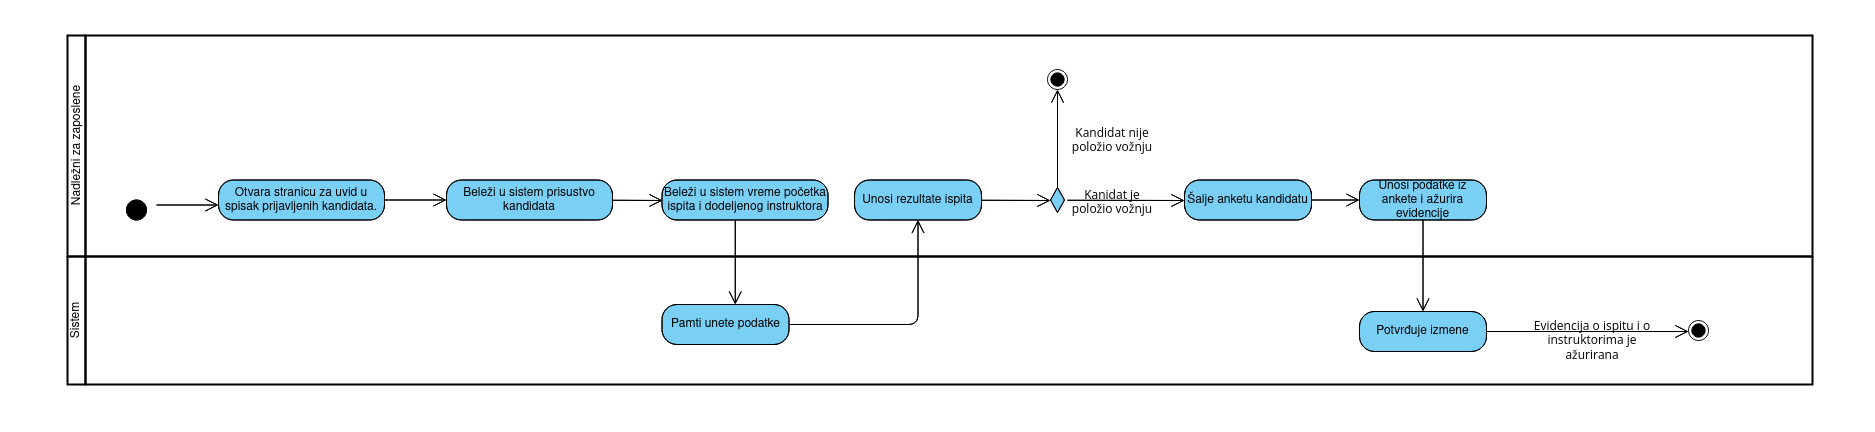
\includegraphics[width=140mm, height=70mm]{Diagrams/dijagram_aktivnosti_vodjenje evidencije.png}
  \end{center}
  \caption {Dijagram aktivnosti - Evidencije o polaganju ispita}
  \label{activity_evidencije_o_polaganju_ispita}

\end{figure}
